
\subsection{BP 7:
 Monai valley beach (Laboratory)}

{\bf Documentation:}  PMEL-135, pp 6 \& 45-46.

\subsubsection{Problems encountered}

\begin{itemize}
\item The input data only goes out to 20 seconds.

\item The first waves are modeled well but later waves are not seen in the
computation.  This is perhaps related to first point.  

\item Data is not provided for run-up in the valley.
\end{itemize}

\subsubsection{What we did}

\begin{itemize}
\item Used $g=9.81$ and no friction.
\item We used the given initial wave to specify a boundary condition at the left
boundary up to time 20.  This was done by filling ghost cells each time step
at the left edge of the computational domain, with cell centers at $x = -
\frac 1 2 \Delta x$ and $x = -\frac 3 2 \Delta x$.
The depth at any such point $x_0$ at arbitrary time $t_0$ should be roughly
the same as the depth at $x=0$ at time $t_0 - x_0/c_0$, where $c_0 =
\sqrt{gh_0}$ is the wave speed based on the constant depth.  This value was
estimated by 
interpolating from the given time trace at $x=0$.
To fully specify the ghost cell values we also need the velocity or momentum
in these cells.  This is estimated by assuming the wave is a right-going
simple wave, so that the Riemann invariant $u - 2\sqrt{gh}$ is constant
through the wave.  Inserting the interpolated $h$ value and then setting this
equal to $-2\sqrt{gh_0}$ gives the expression for the velocity $u$ used in
the ghost cell.

\item After time 20, switched to non-reflecting boundary condition 
at left boundary, so reflected waves exit.  
(Note that the wave tank was much longer than computational domain specified.)
\item We solved on $423\times 243$ grid (same as bathymetry)
\item We also solved on $211\times 121$ grid, coarser by roughly a factor of
2, for comparison as a test of convergence.
\end{itemize} 

\subsubsection{Gauge comparisons}

\Fig{bp7gauges} shows a comparison of the GeoClaw results with the
laboratory values at the three gauges requested, with both grid resolutions. 
The two resolutions give very comparable results, indicating that the
solution presented is close to a converged solution of the shallow water
equations.  The results are in general a good match to the laboratory
measurements.

\begin{figure}[ht]
\hfil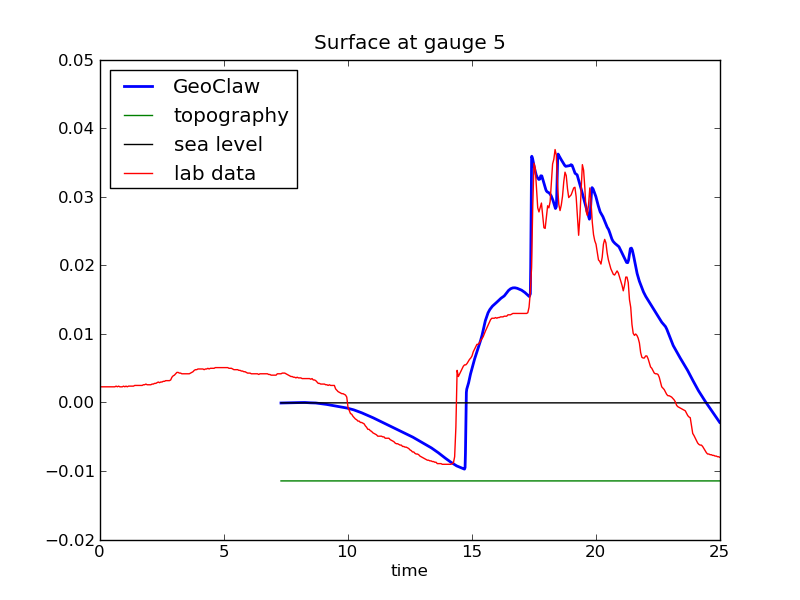
\includegraphics[width=2.8in]{bp7/figs423/gauge0005fig300.png}\hfil
\hfil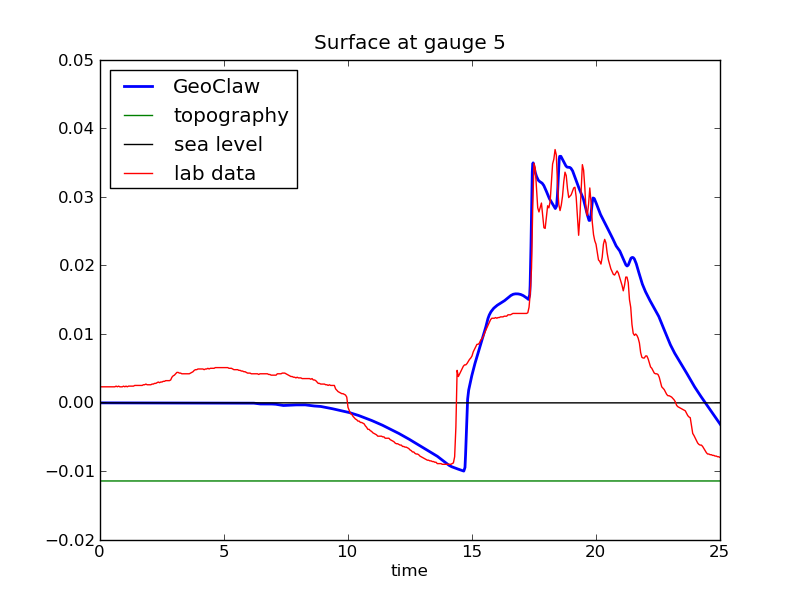
\includegraphics[width=2.8in]{bp7/figs211/gauge0005fig300.png}\hfil
\vskip 5pt
\hfil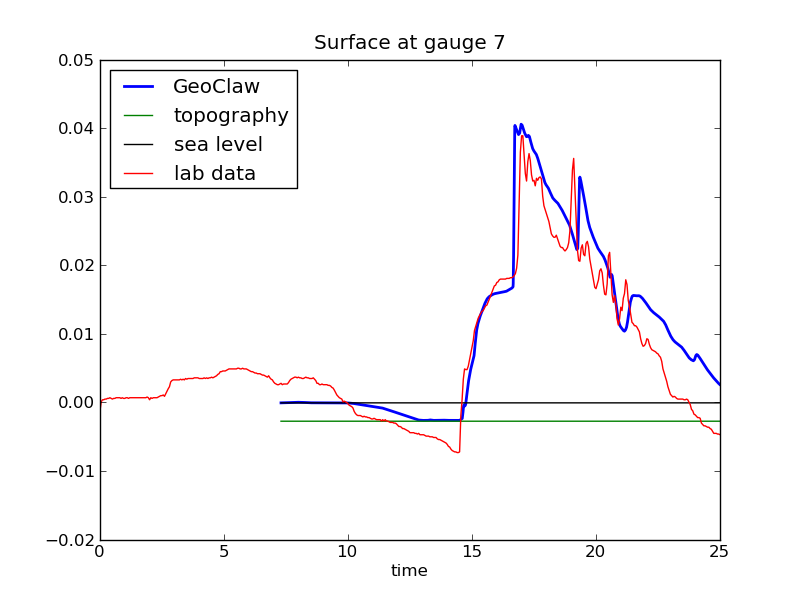
\includegraphics[width=2.8in]{bp7/figs423/gauge0007fig300.png}\hfil
\hfil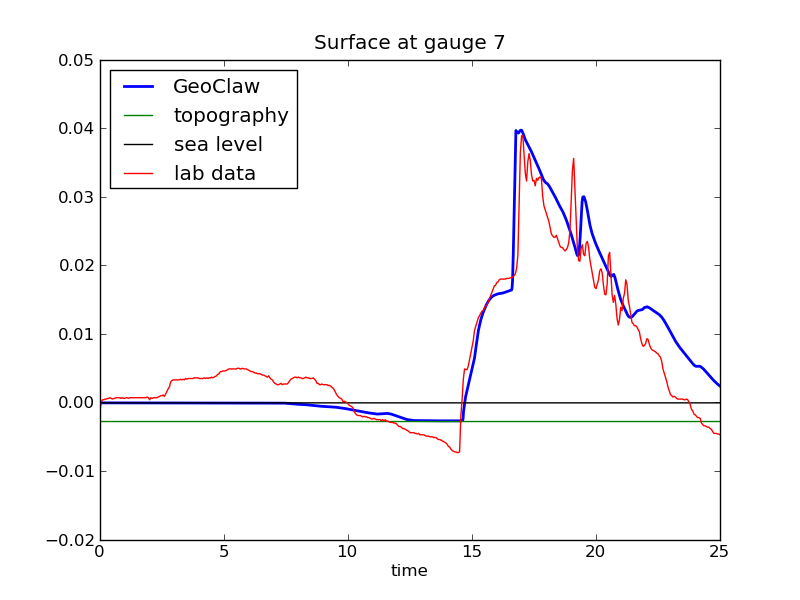
\includegraphics[width=2.8in]{bp7/figs211/gauge0007fig300.png}\hfil
\vskip 5pt
\hfil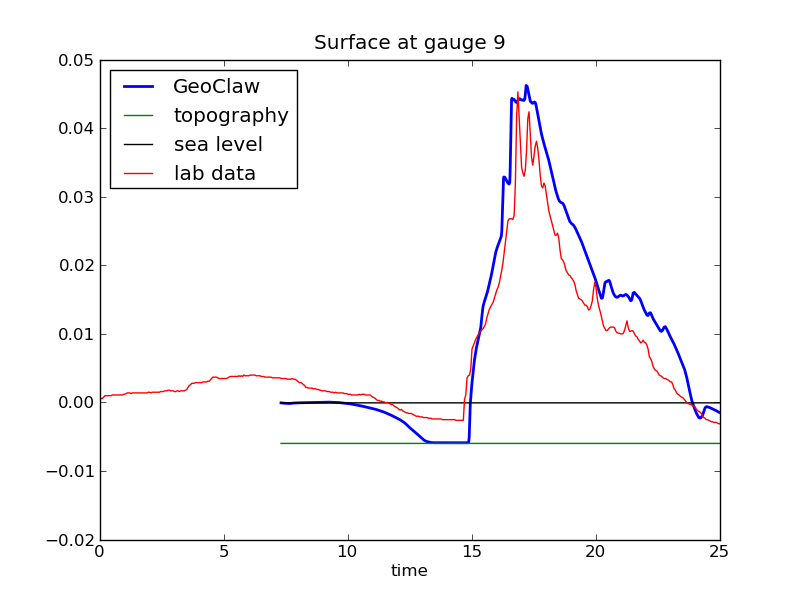
\includegraphics[width=2.8in]{bp7/figs423/gauge0009fig300.png}\hfil
\hfil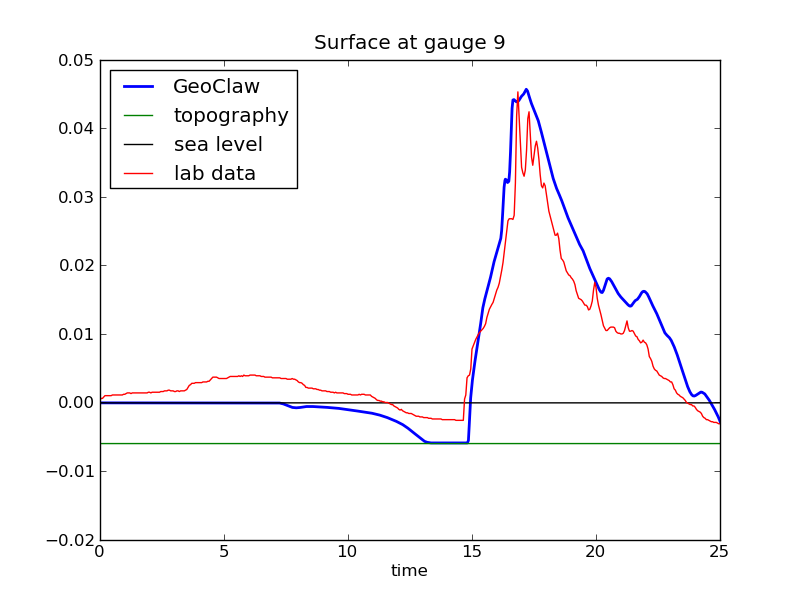
\includegraphics[width=2.8in]{bp7/figs211/gauge0009fig300.png}\hfil
\caption{\label{fig:bp7gauges} 
Left column: on $423\times 243$ grid (same as given bathymetry).
Right column: $211\times 121$ grid.
  }
\end{figure}



\subsubsection{Frame comparisons}

See \Fig{bp7framesA} and \Fig{bp7framesA} for comparisons of the Frames 10,
25, 40, 55, and 70 from the overhead movie with GeoClaw results at roughly
corresponding times.  These results are from the $423\times 243$ grid (same
as given bathymetry).

The movie had a rate of 30 fps, so the frames are 0.5 seconds apart. However,
it is not clear what the starting time was for Frame 1 relative to the
simulation time.   In the Benchmark Description \cite{bp7description}, it is
stated that ``frame 10 approximately occurs at 15.3 seconds'', but then later
``it is recommend that each modeler find times of the snapshots that best fit
the data''.   We found reasonably good agreement starting at 15 seconds for
Frame 1 and then taking 0.5 second increments, as shown in \Fig{bp7framesA}
and \Fig{bp7framesA}.

The yellow dashed lines on the frames from the movie show the approximate
shoreline (and were provided as part of the benchmark specification
\cite{bp7description}).  The actual shoreline location is of course somewhat
ambiguous in the movie, and also in the computation.  The figures of the
GeoClaw computation show the shoreline two different ways:
\begin{itemize}
\item The cells colored blue are finite volume cells where the fluid depth is
greater than 0.0001 m. Those colored green have less fluid or are dry.
\item The black dashed line is a contour line where depth $= 0.002$ m, which
agrees better with the movie frames and might be a depth that can actually be
detected in the movie frames.
\end{itemize} 

\begin{figure}[ht]
\hfil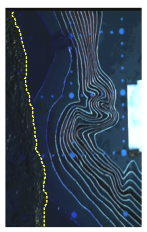
\includegraphics[width=1.5in]{bp7/movie/Frame10.png}\hfil
\hfil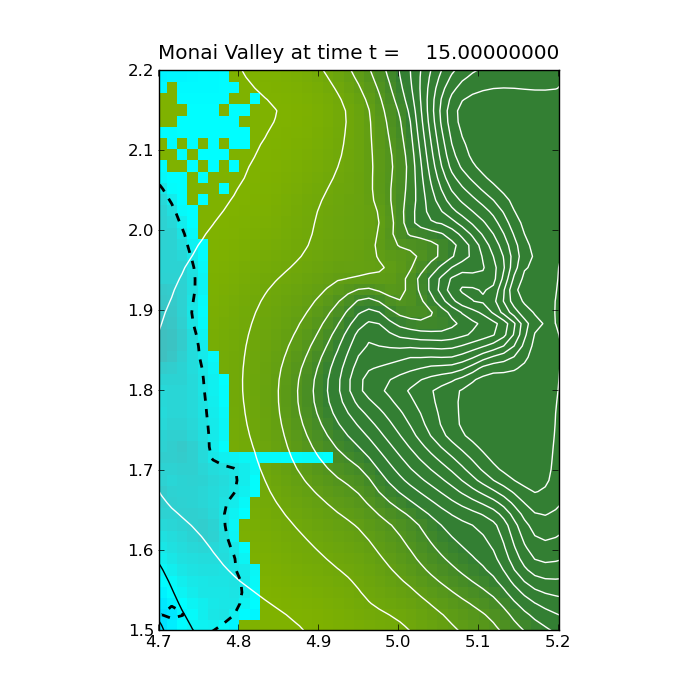
\includegraphics[width=2.8in]{bp7/figs423/frame0005fig10.png}\hfil
\vskip 5pt
\hfil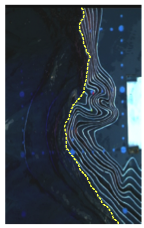
\includegraphics[width=1.5in]{bp7/movie/Frame25.png}\hfil
\hfil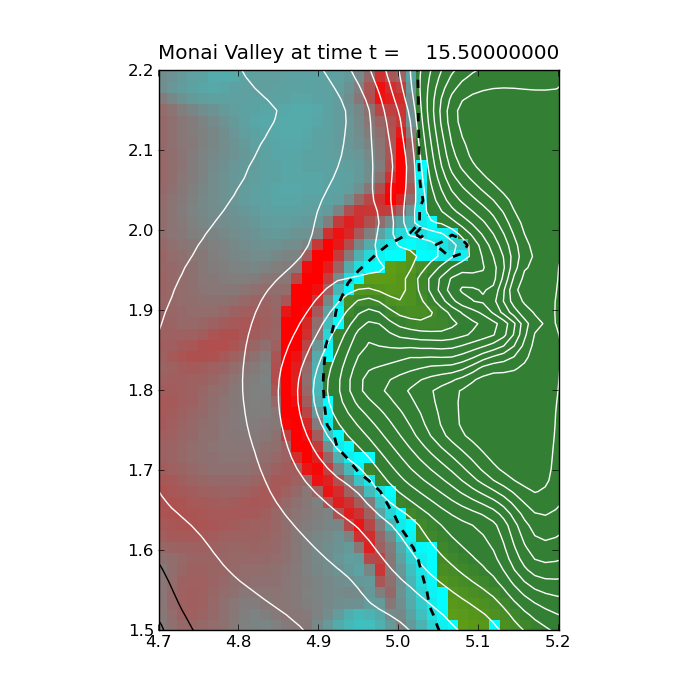
\includegraphics[width=2.8in]{bp7/figs423/frame0007fig10.png}\hfil
\vskip 5pt
\hfil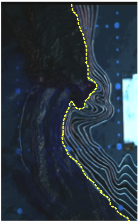
\includegraphics[width=1.5in]{bp7/movie/Frame40.png}\hfil
\hfil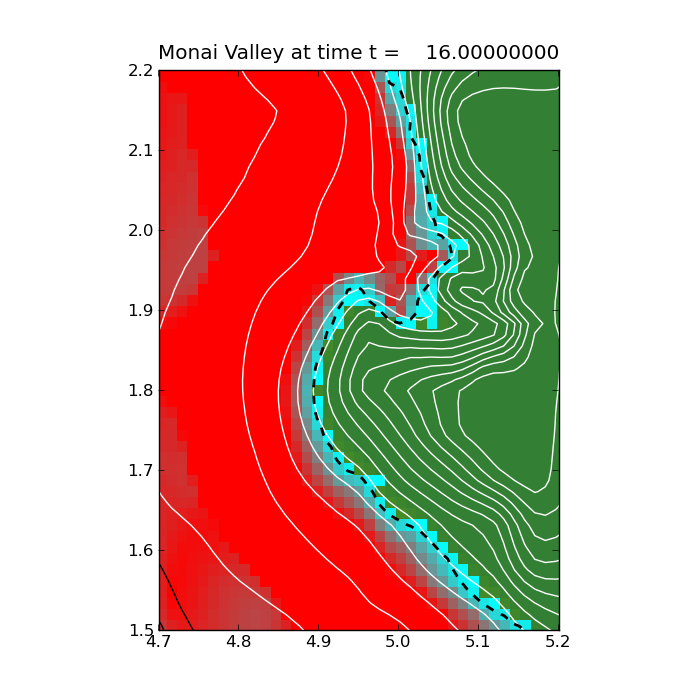
\includegraphics[width=2.8in]{bp7/figs423/frame0009fig10.png}\hfil
\caption{\label{fig:bp7framesA} 
Left column: Frames from the movie.
Right column: Zoomed view of computation.
  }
\end{figure}


\begin{figure}[ht]
\hfil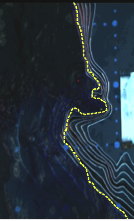
\includegraphics[width=1.5in]{bp7/movie/Frame55.png}\hfil
\hfil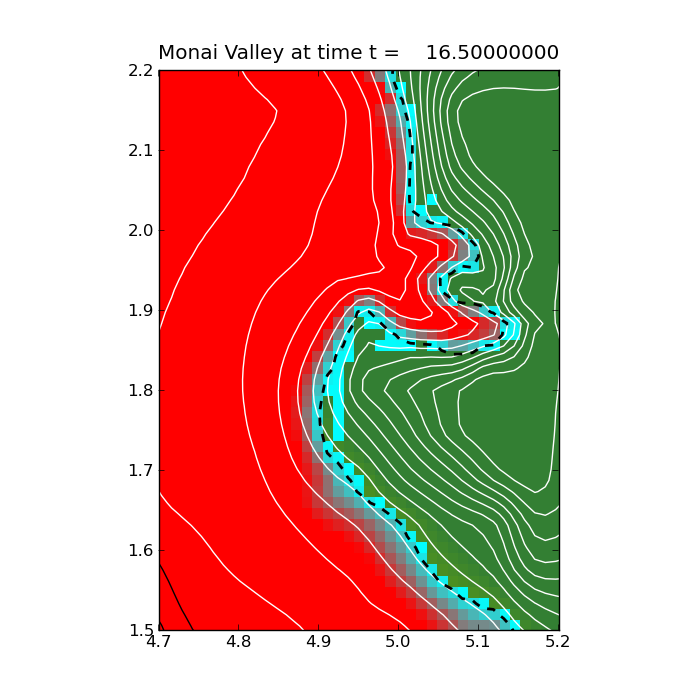
\includegraphics[width=2.8in]{bp7/figs423/frame0011fig10.png}\hfil
\vskip 5pt
\hfil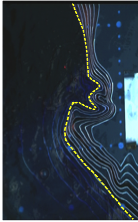
\includegraphics[width=1.5in]{bp7/movie/Frame70.png}\hfil
\hfil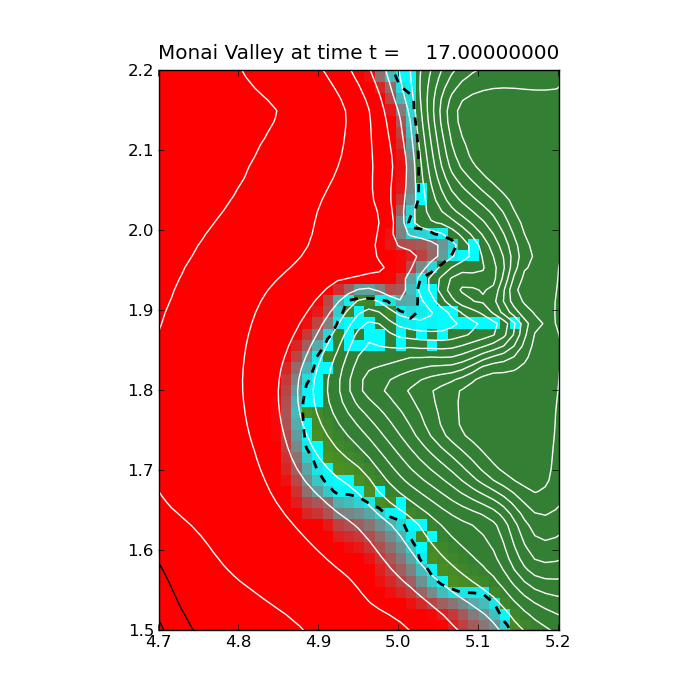
\includegraphics[width=2.8in]{bp7/figs423/frame0013fig10.png}\hfil
\vskip 5pt
\caption{\label{fig:bp7framesB} 
Left column: Frames from the movie.
Right column: Zoomed view of computation.
  }
\end{figure}

\subsection{Runup in the valley}

\subsection{Lessons learned}

\todo{Make any relevant comments or observation regarding the benchmark itself,
the available data provided, the relevance of the benchmark to tsunami
science in general and to validating your specific model in particular. 
Report problems and make recommendations regarding improving the benchmark
or its data, as appropriate.}

